\usepackage{tikz,tikz-cd}
\usetikzlibrary{arrows}
\usetikzlibrary{babel}

\tikzset{%
implies/.style={double,double equal sign distance,-implies},
shorten <>/.style={shorten >=#1,shorten <=#1}}

\newlength{\spacing}
\setlength{\spacing}{0pt}
%
\def\scaling{.2}
%
\newlength{\raising}
\setlength{\raising}{.5pt}

\def\drawboxvoid{
\begin{tikzpicture}[scale=\scaling]
\draw (0,0) rectangle (1,1);%
\end{tikzpicture}}
%%%%%
\def\drawluangle{\begin{tikzpicture}[scale=\scaling]
\draw (0,0) -- (0,1) -- (1,1);%
\end{tikzpicture}}
%%%%%
\def\drawdbluangle{\begin{tikzpicture}[scale=\scaling]
\draw (0,0) -- (0,1) -- (1,1);%
\end{tikzpicture}}
%%%%%
\def\drawrdangle{\begin{tikzpicture}[scale=\scaling]
\draw (0,0) -- (1,0) -- (1,1);%
\end{tikzpicture}}
%%%%%
\def\drawtwoboxes{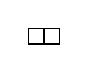
\begin{tikzpicture}[scale=\scaling]
\draw (0,0) -- (1,0) -- (1,1) -- (0,1) -- cycle;%
\draw[xshift=1cm] (0,0) -- (1,0) -- (1,1) -- (0,1) -- cycle;%
\end{tikzpicture}}
%%%%%
\def\drawldangle{\begin{tikzpicture}[scale=\scaling]
\draw (1,0) -- (0,0) -- (0,1);%
\end{tikzpicture}}
%%%%%
\def\drawboxvoidbar{\begin{tikzpicture}[scale=\scaling]
\draw (1,1) -- (1,0) -- (0,0) -- (0,1) -- (2,1);%
\end{tikzpicture}}
%%%%%
\def\boxvoid   {\raisebox{\raising}{\drawboxvoid}}
\def\twoboxes  {\raisebox{\raising}{\drawtwoboxes}}
\def\ldangle   {\raisebox{\raising}{\drawldangle}}
\def\boxvoidbar{\raisebox{\raising}{\drawboxvoidbar}}
\def\luangle{\text{\mbox{$\updownline\hskip-6.13pt\raisebox{4.37pt}{$\leftrightline$}$}}}
\def\rdangle{\text{\mbox{$\raisebox{-4.37pt}{$\leftrightline$}\hskip-6.13pt\updownline$}}}
\def\dbluangle {\raisebox{\raising}{\drawdbluangle}}


\def\leftpull {\boxtimes\hskip-.37em\Box}
\def\leftpush {\boxplus\hskip-.37em\Box}
\def\rightpull{\Box\hskip-.37em\boxtimes}
\def\rightpush{\Box\hskip-.37em\boxplus}
\def\nboxes   {\square\hskip-.16em\square\cdots\square}